\documentclass[11pt,a4paper]{article}
\usepackage[margin=2.5cm]{geometry}
\usepackage{amsmath,amssymb}
\usepackage[authoryear,round]{natbib}
\usepackage{setspace}
\usepackage{graphicx}
\usepackage{booktabs}
\usepackage{float}
\usepackage{tikz}
\onehalfspacing
\graphicspath{{figures/}}
\newcommand{\Bin}{\mathrm{Bin}}
\newcommand{\dd}{\mathrm{d}}
\newcommand{\AI}{\mathrm{AI}}
\newcommand{\Cov}{\mathrm{Cov}}
\newcommand{\Var}{\mathrm{Var}}

\title{Directed Gaussian fields on the river network for the breeding suitability of \textit{Simulium} in a zero-inflated model of onchocerciasis prevalence}
\author{}
\date{}

\begin{document}
\maketitle

\section{Introduction}

In the zero-inflated river-network model for onchocerciasis nodule prevalence in Sudan and South Sudan, the exposure of a village is generated by breeding of blackflies along the rivers within dispersal range, and the suitability of the rivers for breeding beyond what their discharge explains is described by a Gaussian field $u$ on the river network. In earlier work $u$ was a Whittle--Mat\'ern field with Kirchhoff conditions at the vertices \citep{bolin2024}. That field treats the network as undirected and gives every river the same weight where rivers meet, and its variance is twice as large at the ends of the network, the headwater streams that are the main breeding habitat, as an artefact of the vertex conditions. The directed Gaussian fields of \citet{bolin2026dir} offer alternatives with explicit assumptions about how suitability propagates along the network: dependence by distance along the river regardless of direction (tail-down), dependence that follows the flow with discharge-weighted mixing at confluences (tail-up), and their sum. This report defines the three fields through their covariance functions, describes how the models are fitted and which approximations are used, and compares them by profile likelihood, joint estimation of the range and random-fold cross-validation.

\section{Data}

The outcome is the number of individuals with palpable onchocercal nodules among those examined in 900 villages of Sudan and South Sudan surveyed by the Rapid Epidemiological Mapping of Onchocerciasis (REMO), 37{,}831 individuals in total, of whom no positives were found in 550 villages. The river network is HydroRIVERS \citep{lehner2013}, restricted to reaches with a long-term average discharge of at least 0.1~m$^3$/s, over the two countries and a margin around them: 478{,}526~km of river, with 32{,}510 headwater sources and 754 outlets. The reach into which each reach flows joins the reaches at confluences and orients the network along the flow. Aridity is the ratio of annual precipitation to reference evapotranspiration from the Global Aridity Index, version~3.1 \citep{zomer2022}, averaged within 2~km of each village.

\section{The zero-inflated river-network model}

Let $x_1, \dots, x_m$ be the villages, with $n_i$ individuals examined and $y_i$ positive at $x_i$, and let $\Gamma$ be the river network. The breeding intensity at a point $s \in \Gamma$ is
\[
w(s) = \exp\{\theta \log Q(s) + u(s)\},
\]
where $Q(s)$ is the discharge of the reach and $u$ is a zero-mean Gaussian field on $\Gamma$. The exposure of a location $x$ is the breeding within reach of it, weighted by straight-line distance,
\[
E(x) = \int_\Gamma \frac{1}{c\,\phi}\, k\!\left(\frac{\lVert x - s\rVert}{\phi}\right) w(s)\, \dd s, \qquad k(t) = (1 - t)_+^4(1 + 4t),
\]
with the Wendland function $k$ \citep{wendland1995}, $c = 2/3$, so that a straight river through $x$ with $w \equiv 1$ gives $E(x) = 1$, and the dispersal range fixed at $\phi = 40$~km \citep{carnaghi2024}. Every stretch of every river within 40~km of a location contributes, whether or not the rivers are connected, with weight $k$ equal to 0.88 at 5~km, 0.63 at 10~km, 0.19 at 20~km and 0.02 at 30~km. A village lies in a zone of local transmission with probability $\pi(x)$, and within a zone the prevalence is $p(x) = 1 - \exp\{-\lambda(x)\}$, with
\[
\mathrm{logit}\,\pi(x) = a_0 + a_E \log E(x) + a_1 \log \AI(x), \qquad
\log \lambda(x) = b_0 + \gamma \log E(x) + b_1 \log \AI(x) + Z(x),
\]
where $Z(x_i) \sim N(0, \sigma_Z^2)$ are independent village effects, and
\[
P(Y_i = 0) = 1 - \pi(x_i) + \pi(x_i)\{1 - p(x_i)\}^{n_i}, \qquad P(Y_i = y) = \pi(x_i) \binom{n_i}{y} p(x_i)^y \{1 - p(x_i)\}^{n_i - y} \quad (y > 0).
\]
Locations more than 40~km from every river have $E = 0$ and are given $\pi = \lambda = 0$. The models compared in this report differ only in the covariance of $u$.

\section{Breeding fields on the river network}

For two points $s, t \in \Gamma$, let $d(s, t)$ be the distance between them along the network, the length of the shortest path through the rivers, which for points on different tributaries runs through the confluence where they meet. Write $t \rightsquigarrow s$ when $s$ is downstream of $t$, so that water flows from $t$ to $s$; two points on different tributaries above their confluence are not flow-connected. Every field below is, along any single stretch of river without confluences, a stationary Ornstein--Uhlenbeck process with variance $\sigma_u^2$ and correlation
\[
\rho(d) = \exp(-2d/r)
\]
at distance $d$ along the river, so that $r$ is the practical range, the distance at which the correlation falls to $e^{-2} \approx 0.14$. The fields differ only in what happens where rivers meet, and hence in the covariance between points on different stretches. In each case the field is defined by a recursion along the edges of the network: the network is represented by a graph with a vertex at each end of every reach and additional vertices so that no edge is longer than 5~km (145{,}329 vertices and 144{,}575 edges), and along an edge of length $\ell$ the value at one end is $e^{-2\ell/r}$ times the value at the other plus independent noise with variance $\sigma_u^2(1 - e^{-4\ell/r})$. Subdividing an edge leaves the field unchanged, so the representation is exact.

Figure~\ref{fig:junction} shows the simplest confluence, two tributaries $A$ and $B$ joining to form $C$, and summarises what each field assumes there.

\begin{figure}[H]
\centering
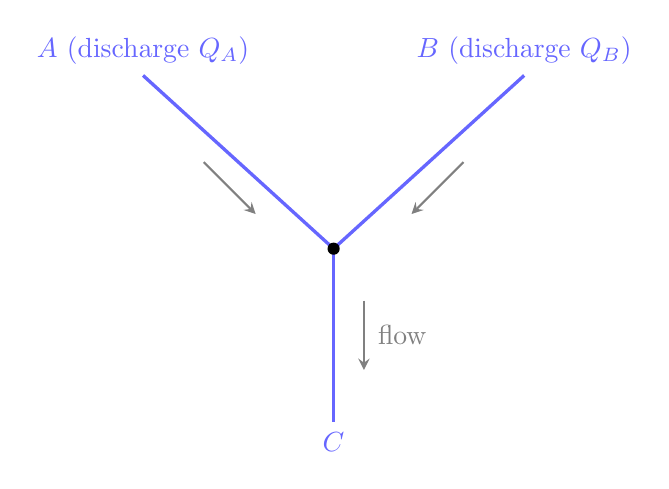
\begin{tikzpicture}[scale=1.1, >=stealth]
  \draw[very thick, blue!60] (-2.2,2) -- (0,0) node[pos=0.0, above] {$A$ (discharge $Q_A$)};
  \draw[very thick, blue!60] (2.2,2) -- (0,0) node[pos=0.0, above] {$B$ (discharge $Q_B$)};
  \draw[very thick, blue!60] (0,0) -- (0,-2) node[pos=1, below] {$C$};
  \draw[->, thick, gray] (-1.5,1.0) -- (-0.9,0.4);
  \draw[->, thick, gray] (1.5,1.0) -- (0.9,0.4);
  \draw[->, thick, gray] (0.35,-0.6) -- (0.35,-1.4);
  \node[gray, right] at (0.4,-1.0) {flow};
  \fill (0,0) circle (2pt);
\end{tikzpicture}
\caption{A confluence. Tail-down: $A$, $B$ and $C$ are correlated by distance along the river, $A$ and $B$ through the confluence. Tail-up: $C$ starts from $\{Q_A u(A^-) + Q_B u(B^-)\}/(Q_A + Q_B)$, where $u(A^-)$ and $u(B^-)$ are the values at the downstream ends of $A$ and $B$; $A$ and $B$ are independent. Symmetric Whittle--Mat\'ern: $A$, $B$ and $C$ meet with the same weight whatever their discharge, and the variance at the confluence is smaller, and at the free ends of $A$ and $B$ larger, than along the rivers.}
\label{fig:junction}
\end{figure}

\subsection*{The symmetric Whittle--Mat\'ern field and why it is no longer used}

The Whittle--Mat\'ern field with $\alpha = 1$ \citep{bolin2024} solves $(\kappa^2 - \Delta_\Gamma)^{1/2}\tau u = \mathcal{W}$ with Kirchhoff conditions at the vertices, continuity of $u$ and zero sum of the outward derivatives. Its precision at the vertices is the sum over edges of length $\ell$ of
\[
\frac{1}{\sigma_u^2(1 - \rho_\ell^2)}\begin{pmatrix} (1 + \rho_\ell^2)/2 & -\rho_\ell \\ -\rho_\ell & (1 + \rho_\ell^2)/2 \end{pmatrix}, \qquad \rho_\ell = e^{-2\ell/r}.
\]
The field ignores the direction of flow and gives every edge meeting at a vertex the same weight, so that a small seasonal stream and the Nile influence each other equally at their confluence. Its variance is not constant: it is $2\sigma_u^2$ at a free end of the network and $2\sigma_u^2/\deg(v)$ near a vertex of degree $\deg(v)$, as an artefact of the Kirchhoff conditions. With 32{,}510 headwater ends, the prior variance of $u$ is twice as large on the small streams as on the rivers they feed, without biological reason. This field is therefore not considered further.

\subsection*{Tail-down field}

The tail-down field is obtained from the directed construction of \citet{bolin2026dir} with every edge reversed, so that the recursion runs upstream from each outlet. The value at each outlet is $N(0, \sigma_u^2)$, and moving upstream along an edge of length $\ell$,
\[
u(\text{upstream end}) = e^{-2\ell/r}\, u(\text{downstream end}) + \varepsilon, \qquad \varepsilon \sim N\{0, \sigma_u^2(1 - e^{-4\ell/r})\}.
\]
At a confluence, seen from downstream, the field divides: both tributaries start from the value at the confluence. The field is continuous, its variance is $\sigma_u^2$ everywhere, and for any two points on the same connected network
\[
\Cov\{u(s), u(t)\} = \sigma_u^2 \exp\{-2\,d(s, t)/r\},
\]
including points on different tributaries, whose distance runs through their confluence; points on different river systems, with different outlets, are independent. This is the exponential tail-down model of \citet{verhoef2010}. Its assumptions are that suitability is similar for stretches of river that are close along the network, irrespective of the direction of flow, and that the strength of this similarity does not depend on the size of the rivers. Because its variance is the same everywhere, it has none of the artefacts of the symmetric field at the river ends and confluences, and on a straight river the two fields coincide.

\subsection*{Tail-up field with discharge-weighted mixing}

The tail-up field runs the recursion in the direction of flow, from the sources. The value at each source is $N(0, \sigma_u^2)$, and moving downstream along an edge,
\[
u(\text{downstream end}) = e^{-2\ell/r}\, u(\text{upstream end}) + \varepsilon, \qquad \varepsilon \sim N\{0, \sigma_u^2(1 - e^{-4\ell/r})\}.
\]
At a confluence of incoming edges $k = 1, \dots, K$, the outgoing river starts from the discharge-weighted average of the incoming values,
\[
u(\text{start of outgoing edge}) = \sum_{k=1}^K p_k\, u(\text{end of incoming edge } k), \qquad p_k = \frac{Q_k}{\sum_{j} Q_j},
\]
the flow-weighted condition K1 of \citet{bolin2026dir}, with the long-term average discharge of the incoming reaches as weights ($\omega = 1$ in the weights $Q^\omega$). The incoming values at a confluence are distinct, so the field can be discontinuous there. On a network oriented along the flow, as HydroRIVERS is, the covariance is
\[
\Cov\{u(s), u(t)\} = \begin{cases} \Var\{u(t)\}\, \exp\{-2\,d(s, t)/r\} \prod_{v} p_v, & t \rightsquigarrow s, \\ 0, & \text{if neither point is downstream of the other,} \end{cases}
\]
where the product is over the confluences $v$ passed between $t$ and $s$ and $p_v$ is the share of the discharge at $v$ carried by the branch containing $t$. The variance is $\sigma_u^2$ above every confluence; just below a confluence of independent tributaries it is $\sigma_u^2 \sum_k p_k^2$, and it returns towards $\sigma_u^2$ downstream. The assumptions are that suitability behaves like a property carried by the water, such as temperature, oxygen or suspended food particles, mixing at confluences in proportion to discharge, and that stretches of river that are not connected by flow are unrelated, however close they are. A small tributary therefore barely affects the main river below it, and two neighbouring tributaries share information only through what they pass downstream.

\subsection*{Sum of tail-up and tail-down fields}

The third field is the sum of independent tail-up and tail-down fields,
\[
u = u_{\uparrow} + u_{\downarrow}, \qquad \Cov\{u(s), u(t)\} = \phi_\uparrow\, C_\uparrow(s, t; r_\uparrow) + (1 - \phi_\uparrow)\, C_\downarrow(s, t; r),
\]
where $C_\uparrow$ and $C_\downarrow$ are the tail-up and tail-down covariances above with variance $\sigma_u^2$, $\phi_\uparrow$ is the share of the variance carried by the tail-up part, and each part has its own range. This model contains the other two as the special cases $\phi_\uparrow = 0$ and $\phi_\uparrow = 1$, and lets the data decide how much of the variation in suitability is shared by neighbouring streams and how much is carried downstream.

For all three fields the recursions make $u$ a Markov field on the graph, with sparse precision matrix
\[
Q = L^\top W L,
\]
where each row of $L$ expresses one value as its recursion residual, with entries 1, $-e^{-2\ell/r}$ and, for the tail-up field, $-e^{-2\ell/r} p_k$ at confluences, and $W$ is diagonal with the inverse noise variances, $1/\sigma_u^2$ at the outlets or sources and $1/\{\sigma_u^2(1 - e^{-4\ell/r})\}$ for the edges. For the tail-down field the latent vector holds the value at each vertex; for the tail-up field it holds the value at each source and at the downstream end of each edge, so that the incoming values at a confluence are separate (177{,}085 values), and the value at any point of an edge is interpolated between its upstream value, which is a discharge-weighted combination of incoming values at a confluence, and its downstream value. The quadrature nodes used for the exposure lie on the edges, and $u$ at a node is the linear interpolation of the values at the two ends of its edge.

\section{Estimation and approximations}

For given values of the parameters $\psi = (\sigma_u, \sigma_Z, a_E, \gamma, r)$, and for the summed field also $\phi_\uparrow$ and $r_\uparrow$, the latent vector, consisting of the regression coefficients $a_0, a_1, b_0, b_1$, the breeding coefficient $\theta$, the values of $u$ on the graph and the village effects, is integrated out by a Laplace approximation. The regression coefficients have independent Gaussian priors with standard deviation 10. The mode of the latent vector is found by Newton's method, with each Newton system solved by conjugate gradients using exact products with the Hessian of the log posterior \citep{steihaug1983}, including the curvature of $\log E$ in $\theta$ and $u$, and preconditioned by the Gauss--Newton Hessian, which is inverted with the Woodbury identity and a sparse Cholesky factor of $Q$. The posterior is approximated by a Gaussian at the mode, and the approximate marginal likelihood is $\log p(y \mid \hat\xi) + \log p(\hat\xi) - \tfrac12 \log\det H(\hat\xi)$, where $\hat\xi$ is the mode and $H$ the negative Hessian; by the matrix determinant lemma the determinant reduces to that of a matrix of dimension $2m$, since each village enters through two linear predictors, $\mathrm{logit}\,\pi(x_i)$ and $\log\lambda(x_i)$. In this Hessian, the observed information of the two predictors of each village is bounded away from zero.

The parameters $\psi$ are estimated by maximising the approximate marginal likelihood with a trust-region Newton method, with derivatives by central finite differences, a full Hessian at the first iteration and BFGS updates thereafter. The coefficients $a_E$ and $\gamma$ are treated as parameters rather than latent effects because they multiply $\log E$, which depends on the latent field. For the range of $u$, the approximate likelihood was profiled over a grid, seven values from 100 to 6{,}400~km for the tail-down field and from 25 to 3{,}200~km for the tail-up field, with the other parameters maximised at each value, and the profile was interpolated by a natural cubic spline in $\log r$ to locate its maximum and an approximate 95\% interval, the values of $r$ at which the profile is 1.92 units below its maximum. The range was then estimated jointly with the other parameters, starting from the best grid value. For the summed field the two ranges, the variance share $\phi_\uparrow$ and the other parameters were estimated jointly, starting from the tail-down estimates with $\phi_\uparrow = 0.05$ and the tail-up range at the maximum of the tail-up profile.

For the tail-up field the posterior of the latent effects has more than one mode: at the same parameter values, a search started from zero reached a mode with log posterior 7.3 units lower, and approximate log-likelihood 16 units lower, than a search started from the mode of a neighbouring fit, and the two modes differ substantially in $u$ and $\theta$. The Laplace approximation describes only the mode it is built on. The search was therefore started from the modes of neighbouring fits and, at each evaluation, from both the latest and the best mode found so far, keeping the higher one. For the tail-down field, searches started from zero and from perturbed modes reached the same mode, with approximate log-likelihoods within 0.1 of each other.

Predictions were assessed by ten-fold cross-validation with villages assigned to folds at random. In each fold the latent effects were refitted to the training villages with the parameters $\psi$ fixed at their estimates from all the data, and the predictive distribution of the number of positives at each held-out village was obtained from the Gaussian approximation to the posterior of its two linear predictors, a new village effect and the zero-inflated binomial distribution, by two-dimensional Gauss--Hermite quadrature. The assessment combines the mean logarithmic score of the predictive distributions, the area under the ROC curve and Brier score of the predicted probability of at least one positive, the expected number of villages without positives, and, among villages with at least one positive, the non-randomised probability integral transform (PIT) of \citet{czado2009}, applied to the predictive distribution conditional on $Y \geq 1$, with its expected variation under calibration from 500 simulations.

The main approximations are therefore the Laplace approximation to the integral over the latent effects, whose accuracy has not been checked and may differ between fields; the use of plug-in estimates of $\psi$, whose uncertainty is not propagated to the standard errors of the regression coefficients or to the predictions; the outer optimisation, which stops within a few tenths of a unit of the maximum on flat directions; and, in the cross-validation, the fixing of $\psi$ at the estimates from all the data, which is slightly optimistic for all models alike. The quadrature for the exposure (nodes at most 2~km apart along the rivers) and the linear interpolation of $u$ within edges of at most 5~km are numerically minor for ranges of hundreds of kilometres. Differences in approximate log-likelihood of one unit or less should be regarded as within the numerical error.

\section{Results}

Figure~\ref{fig:profiles} shows the profile likelihoods. The tail-down profile rises steeply up to about 400~km and has a broad, flat maximum: the interpolated maximum is at 1{,}357~km, with an approximate 95\% interval from 434 to 2{,}602~km, and the joint estimate, 1{,}017~km, lies on the same plateau, 0.07 units below the interpolated maximum. The tail-up profile is more peaked, with its maximum at 520~km and an interval from 377 to 767~km; its joint estimate is 514~km. At every range the tail-down field fits better than the tail-up field, by 27 units at their respective maxima. With a correlation of $e^{-2}$ at about 1{,}000~km along the river, the tail-down field changes little along a tributary system and mainly between sub-basins; because distance is measured along the network, through the confluence, two streams a few kilometres apart on the ground may be several hundred kilometres apart along the rivers, and it is this long range that lets neighbouring streams share information.

\begin{figure}[H]
\centering
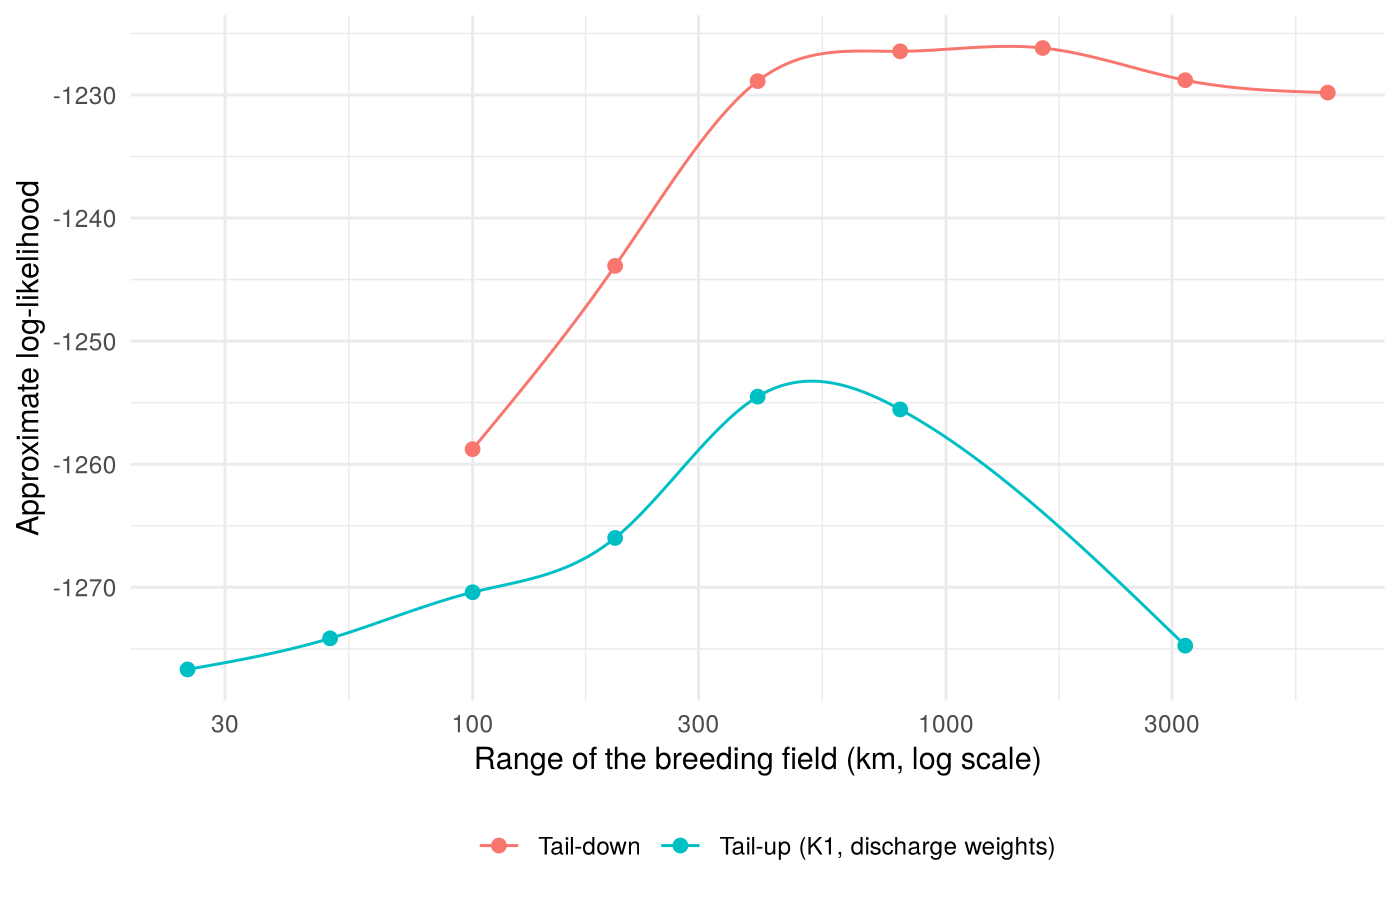
\includegraphics[width=0.72\textwidth]{directed_profiles.png}
\caption{Profile approximate log-likelihood over the range of the breeding field, for the tail-down and tail-up fields; each point is maximised over the other parameters, and the curves are natural cubic splines in $\log r$.}
\label{fig:profiles}
\end{figure}

Table~\ref{tab:estimates} gives the joint estimates. The tail-down field and the summed field give practically the same estimates: in the summed field the tail-up part carries 5\% of the variance, its range stayed at its starting value of 200~km, along which the likelihood is flat, and the approximate log-likelihood is 0.8 units higher than for the tail-down field alone, within the numerical error. The tail-up field fits worse and changes the other estimates: the effects of aridity are stronger in both parts of the model ($a_1 = 3.62$ against 1.89, $b_1 = 0.95$ against 0.53), the coefficients of exposure are larger ($a_E = 0.88$ against 0.50, $\gamma = 0.19$ against 0.10), the breeding coefficient of discharge changes sign ($\theta = 0.24$ against $-0.48$), and $\sigma_u$ is smaller. Without a shared component for neighbouring streams, the regional contrasts that the tail-down field attributes to the rivers are taken up by aridity and by the exposure coefficients.

\begin{table}[H]
\centering
\caption{Joint estimates (standard errors for the regression coefficients, conditional on the other parameters) and approximate log-likelihood of the zero-inflated model with each breeding field.}
\label{tab:estimates}
\begin{tabular}{lrrr}
\toprule
 & Tail-down & Tail-up (K1) & Tail-up + tail-down \\
\midrule
Range $r$ (km) & 1017 & 514 & 967 (tail-down part) \\
Range $r_\uparrow$ of the tail-up part (km) & -- & -- & 200 \\
Tail-up share of variance $\phi_\uparrow$ & 0 & 1 & 0.05 \\
$\sigma_u$ & 7.47 & 5.47 & 7.47 \\
$\sigma_Z$ & 0.50 & 0.45 & 0.50 \\
\midrule
$a_0$ (intercept, $\mathrm{logit}\,\pi$) & 1.97 (0.93) & 1.90 (0.45) & 1.86 (0.92) \\
$a_1$ ($\log\AI$, $\mathrm{logit}\,\pi$) & 1.89 (0.55) & 3.62 (0.49) & 1.88 (0.54) \\
$a_E$ ($\log E$, $\mathrm{logit}\,\pi$) & 0.50 & 0.88 & 0.50 \\
$b_0$ (intercept, $\log\lambda$) & $-1.61$ (0.19) & $-1.62$ (0.10) & $-1.63$ (0.19) \\
$b_1$ ($\log\AI$, $\log\lambda$) & 0.53 (0.12) & 0.95 (0.11) & 0.53 (0.12) \\
$\gamma$ ($\log E$, $\log\lambda$) & 0.10 & 0.19 & 0.10 \\
$\theta$ ($\log Q$, breeding) & $-0.48$ (0.32) & 0.24 (0.16) & $-0.53$ (0.35) \\
\midrule
Approximate log-likelihood & $-1226.12$ & $-1253.17$ & $-1225.29$ \\
\bottomrule
\end{tabular}
\end{table}

The cross-validation (Table~\ref{tab:cv}) agrees with the likelihood. The tail-down and summed fields have the same scores to the second or third decimal place: the sum of the logarithmic scores over the 900 villages differs by 0.8, the same amount as the approximate log-likelihood. The tail-up field is worse on every measure of discrimination and overall fit: its total logarithmic score is about 20 units lower, its area under the ROC curve and Brier score are worse, the correlation between observed and predicted prevalence is lower, and it predicts 31 villages without positives among the humid villages, against 14 observed and 22 for the tail-down field. Among villages with at least one positive, the PIT histogram of the tail-up field is the flattest (Figure~\ref{fig:pit}), with all ten bins inside their expected range, whereas the tail-down and summed fields each have three bins just outside it, with a slight excess between 0.4 and 0.5 and a deficit between 0.6 and 0.8; this departure is modest and has no clear shape of over- or under-dispersion. The advantage of the tail-down field therefore lies in separating villages with and without transmission, and in predicting where infection occurs, rather than in the calibration of the numbers of positives.

\begin{table}[H]
\centering
\caption{Ten-fold cross-validation with random folds. The total logarithmic score is the sum over the 900 villages of the log predictive probability of the observed count; 550 villages had no positives, 14 of them in the sub-humid and humid class.}
\label{tab:cv}
\begin{tabular}{lrrr}
\toprule
 & Tail-down & Tail-up (K1) & Tail-up + tail-down \\
\midrule
Mean logarithmic score & $-1.301$ & $-1.323$ & $-1.300$ \\
Total logarithmic score & $-1171.1$ & $-1190.8$ & $-1170.3$ \\
Area under the ROC curve & 0.952 & 0.950 & 0.952 \\
Brier score & 0.082 & 0.086 & 0.082 \\
Correlation of observed and predicted prevalence & 0.755 & 0.734 & 0.755 \\
Expected villages without positives (550) & 547.8 & 555.0 & 547.7 \\
\quad of which sub-humid and humid (14) & 22.4 & 30.9 & 22.9 \\
PIT bins outside their 95\% range (of 10) & 3 & 0 & 3 \\
\bottomrule
\end{tabular}
\end{table}

\begin{figure}[H]
\centering
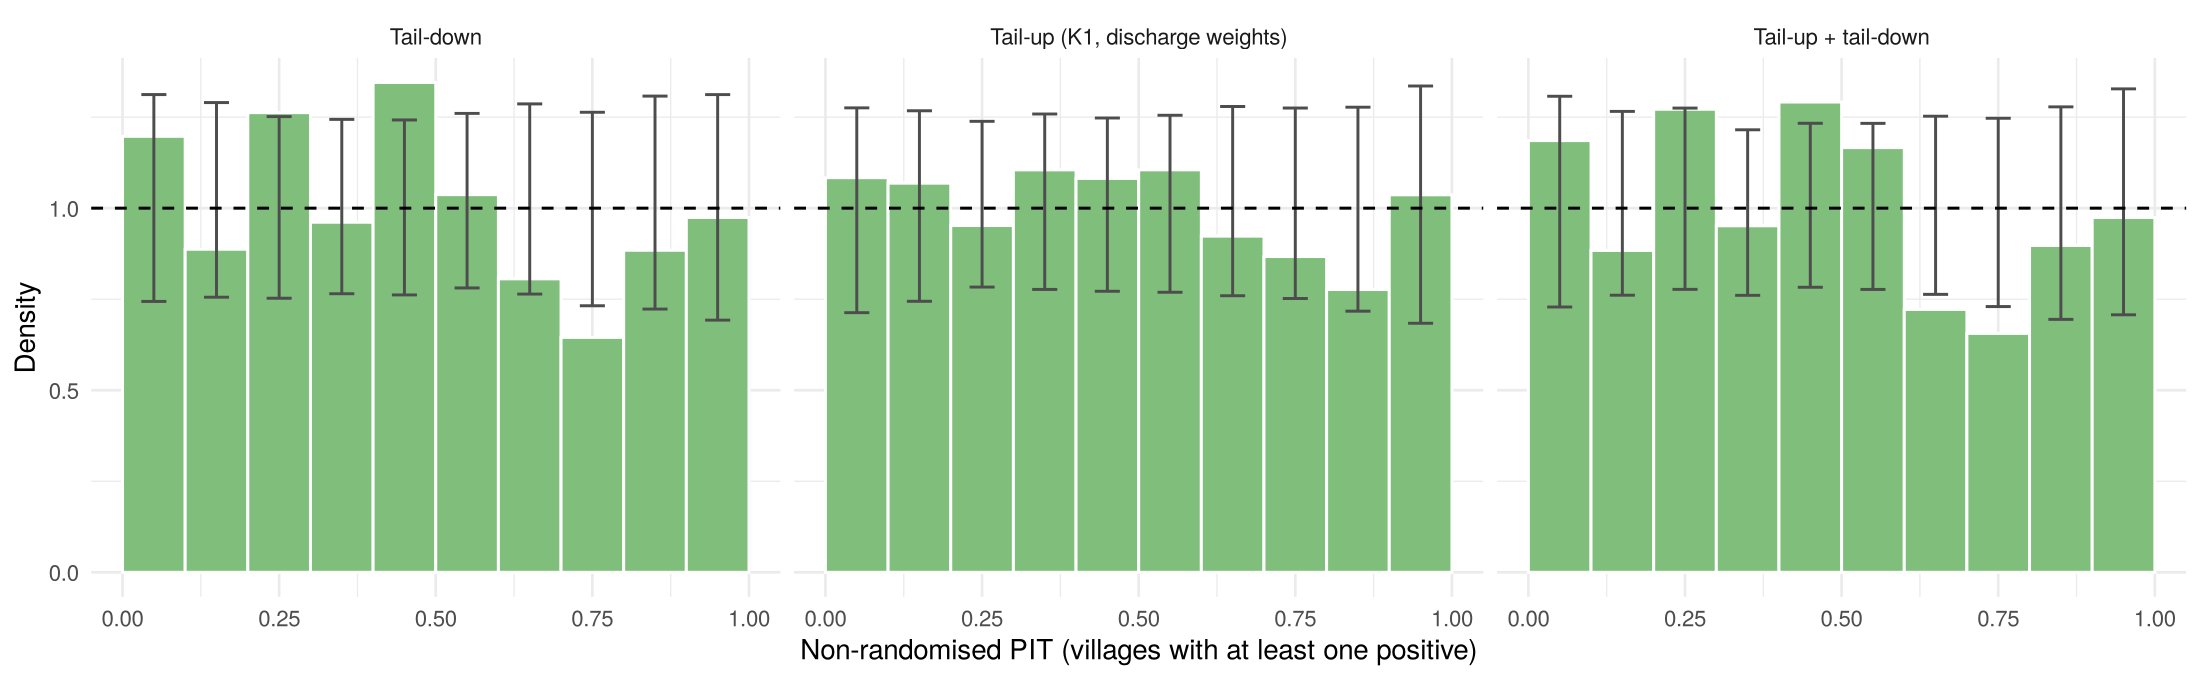
\includegraphics[width=\textwidth]{directed_joint_pit.png}
\caption{Non-randomised PIT \citep{czado2009} among the 350 villages with at least one positive, conditional on $Y \geq 1$, from ten-fold cross-validation with random folds; bars show the 95\% range expected under calibration.}
\label{fig:pit}
\end{figure}

The posterior modes of $u$ (Figure~\ref{fig:umaps}) show what the fields imply. The tail-down field varies smoothly over whole sub-basins: it is high on the Nile between Abu Hamad and the Atbara confluence, where the river crosses the Fourth and Fifth Cataracts, on the tributaries of the Nile in northern Kordofan and Darfur, and over the networks of small streams in the far west and south of South Sudan, and low over the Bahr el Ghazal and its tributaries, the White Nile, and the Blue Nile, Atbara and other rivers of the east. The tail-up field cannot form such regional levels: the high values are confined to the main channel of the Nile and to individual streams in South Sudan, and neighbouring streams have unrelated values, while the Bahr el Ghazal and White Nile carry the low values. The summed field is indistinguishable from the tail-down field.

\begin{figure}[H]
\centering
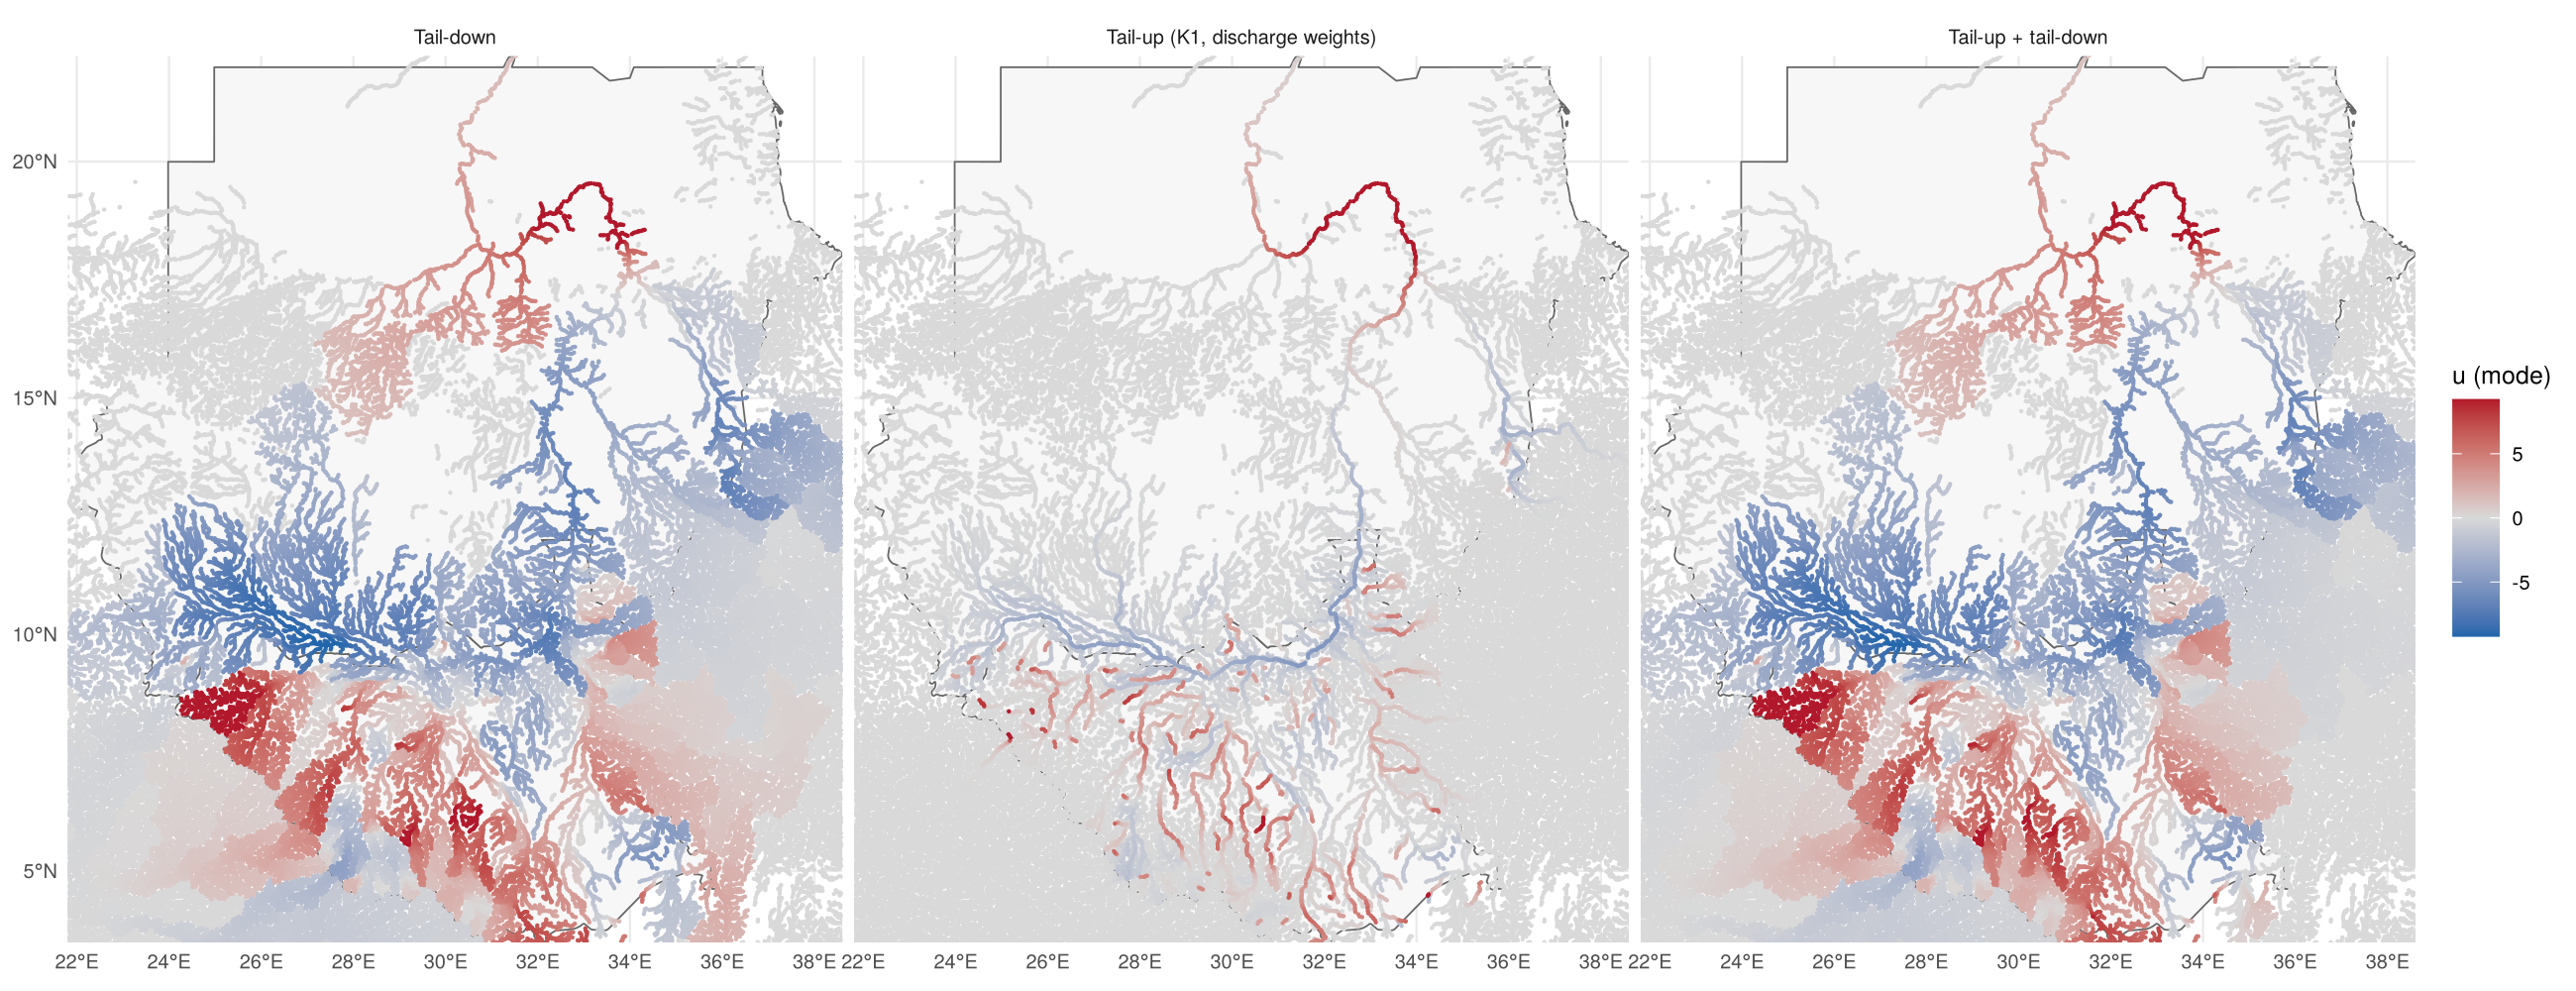
\includegraphics[width=\textwidth]{directed_joint_u_maps.png}
\caption{Posterior mode of the breeding field $u$ (log multiplier of the breeding intensity) along the river network for the joint fits of the three models.}
\label{fig:umaps}
\end{figure}

The maps of expected prevalence (Figure~\ref{fig:prevmaps}) are similar in their broad pattern, with infection predicted in South Sudan and along the southern margin of Sudan and essentially none in the desert. The correlation of expected prevalence over the 20~km grid is 0.998 between the tail-down and summed fields, with a largest difference of 0.11, and 0.91 between the tail-down and tail-up fields. The tail-up map is patchier, following individual streams, and its predictions are lower in the north of South Sudan and higher in a few foci in the west.

\begin{figure}[H]
\centering
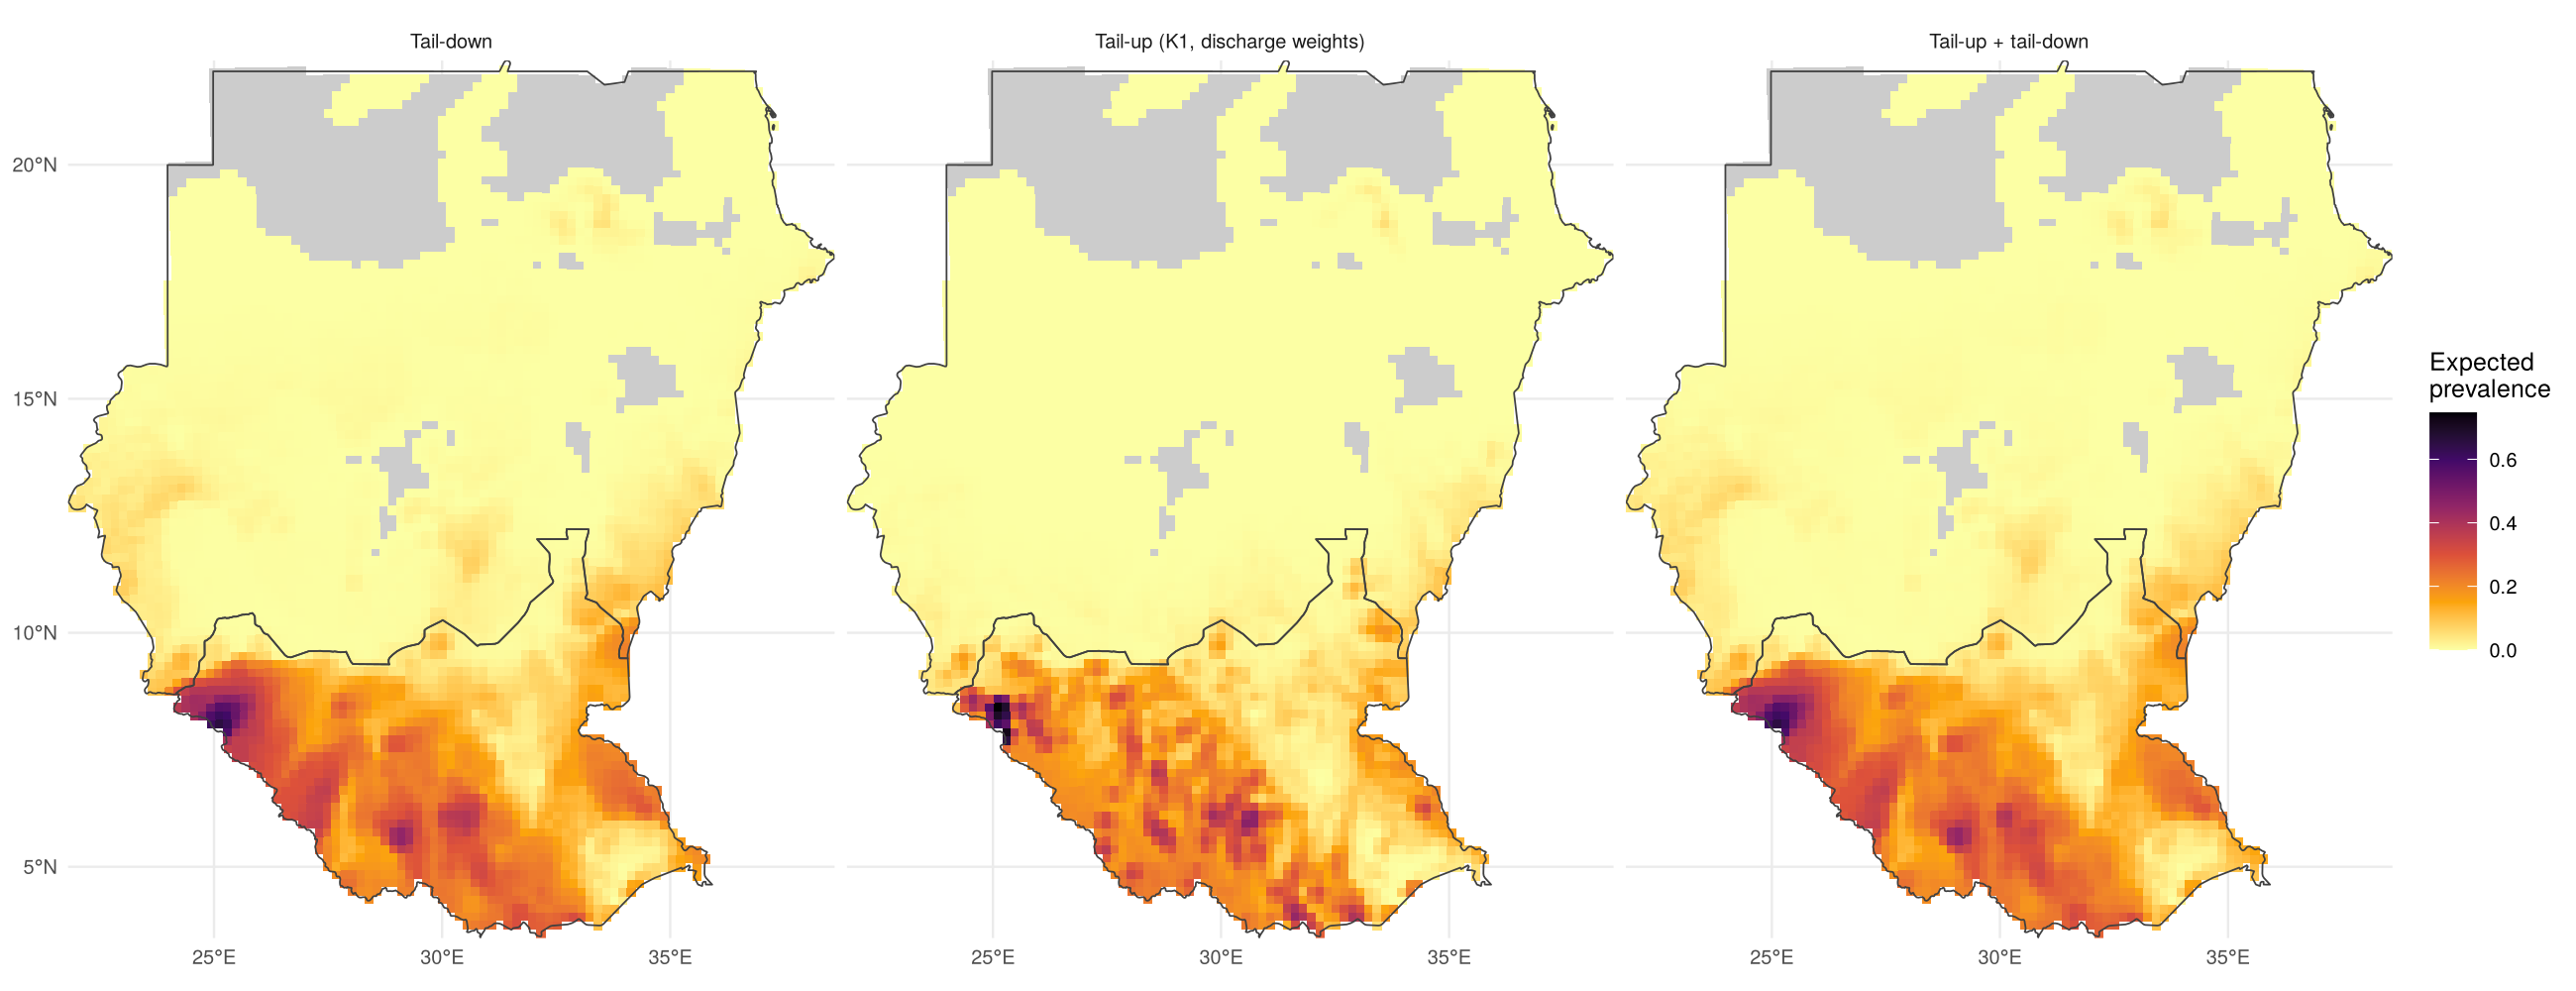
\includegraphics[width=\textwidth]{directed_joint_prevalence_maps.png}
\caption{Expected prevalence $\pi(x)p(x)$ on a 20~km grid, at the posterior mode with the village effect set to zero, for the three models; grey cells lie more than 40~km from every river reach.}
\label{fig:prevmaps}
\end{figure}

\section{Discussion}

Of the three directed fields, the tail-down field describes the data best. Allowing part of the variation in breeding suitability to follow the flow, with discharge-weighted mixing at confluences, does not improve the fit: in the summed field the data give the tail-up part 5\% of the variance and a gain in approximate log-likelihood and in cross-validated logarithmic score of less than one unit. On its own, the tail-up field fits worse by 27 units, predicts worse, and changes the estimated effects of aridity, exposure and discharge in compensation. The suitability of the rivers for breeding therefore appears to be shared by neighbouring streams, whether or not they are connected by flow, and to vary mainly between sub-basins, as expected if it reflects terrain, geology and climate rather than properties carried by the water. Compared with the symmetric Whittle--Mat\'ern field used before, the tail-down field has the same interpretation without the inflated variance at the river ends.

Several limitations remain. The comparisons rest on Laplace approximations, whose accuracy was not checked and may differ between fields; for the tail-up field the latent posterior has several modes, and the reported fit uses the highest mode found. The range of the tail-down field is weakly determined, between about 400 and 2{,}600~km, which matters little for the predictions but means that its value should not be interpreted too precisely. The weights at confluences were fixed at the long-term average discharge; weights $Q^\omega$ with $\omega$ estimated, or the dry-season discharge, could be considered, although with the tail-up part receiving 5\% of the variance this is unlikely to change the conclusions. Finally, measured characteristics of the rivers, such as channel gradient as a proxy for water velocity, the permanence of flow and the presence of lakes and reservoirs upstream, could explain part of the field $u$ and are the natural next step.

\begin{thebibliography}{9}

\bibitem[Bolin et al.(2024)]{bolin2024}
Bolin, D., Simas, A.~B. and Wallin, J. (2024).
\newblock Gaussian Whittle--Mat\'ern fields on metric graphs.
\newblock \textit{Bernoulli}, 30(2), 1611--1639.

\bibitem[Bolin et al.(2026)]{bolin2026dir}
Bolin, D., Simas, A.~B., Karlsson Strandh, E. and Wallin, J. (2026).
\newblock Gaussian processes on directed metric graphs.
\newblock arXiv:2609.01435.

\bibitem[Carnaghi et al.(2024)]{carnaghi2024}
Carnaghi, M. et al. (2024).
\newblock Short- and long-range dispersal by members of the \textit{Simulium damnosum} complex (Diptera: Simuliidae), vectors of onchocerciasis: a review.
\newblock \textit{Insects}, 15(8), 606.

\bibitem[Czado et al.(2009)]{czado2009}
Czado, C., Gneiting, T. and Held, L. (2009).
\newblock Predictive model assessment for count data.
\newblock \textit{Biometrics}, 65, 1254--1261.

\bibitem[Lehner and Grill(2013)]{lehner2013}
Lehner, B. and Grill, G. (2013).
\newblock Global river hydrography and network routing: baseline data and new approaches to study the world's large river systems.
\newblock \textit{Hydrological Processes}, 27, 2171--2186.

\bibitem[Steihaug(1983)]{steihaug1983}
Steihaug, T. (1983).
\newblock The conjugate gradient method and trust regions in large scale optimization.
\newblock \textit{SIAM Journal on Numerical Analysis}, 20(3), 626--637.

\bibitem[Ver Hoef and Peterson(2010)]{verhoef2010}
Ver Hoef, J.~M. and Peterson, E.~E. (2010).
\newblock A moving average approach for spatial statistical models of stream networks.
\newblock \textit{Journal of the American Statistical Association}, 105(489), 6--18.

\bibitem[Wendland(1995)]{wendland1995}
Wendland, H. (1995).
\newblock Piecewise polynomial, positive definite and compactly supported radial functions of minimal degree.
\newblock \textit{Advances in Computational Mathematics}, 4, 389--396.

\bibitem[Zomer et al.(2022)]{zomer2022}
Zomer, R.~J., Xu, J. and Trabucco, A. (2022).
\newblock Version 3 of the Global Aridity Index and Potential Evapotranspiration Database.
\newblock \textit{Scientific Data}, 9, 409.

\end{thebibliography}

\end{document}
